\documentclass[aspectratio=169,11pt]{beamer}
\usepackage[utf8]{inputenc}
\usepackage[T1]{fontenc}
\usepackage{lmodern,graphicx,amsmath,amssymb,booktabs,array}
\usepackage{xcolor,tikz}
\usetikzlibrary{arrows.meta,positioning,calc,fit,shapes.geometric}

% -----------------------------------------------------------------------------
% TUM-inspired visual language matching the supplied presentation.
\definecolor{tumblue}{RGB}{0,101,189}
\definecolor{tumdark}{RGB}{0,51,89}
\definecolor{tumgray}{RGB}{105,105,105}
\definecolor{tumlight}{RGB}{235,243,248}
\definecolor{tumgreen}{RGB}{162,173,0}
\definecolor{tumorange}{RGB}{243,125,32}
\definecolor{tumred}{RGB}{229,52,24}
\definecolor{modelgreen}{HTML}{4C956C}
\definecolor{datagray}{HTML}{E8E8E8}

\usetheme{default}
\setbeamertemplate{navigation symbols}{}
\setbeamercolor{normal text}{fg=black,bg=white}
\setbeamercolor{frametitle}{fg=tumblue}
\setbeamercolor{structure}{fg=tumblue}
\setbeamercolor{itemize item}{fg=tumblue}
\setbeamercolor{block title}{fg=white,bg=tumblue}
\setbeamercolor{block body}{fg=black,bg=tumlight}
\setbeamertemplate{itemize items}[circle]

% TUM logo on every slide. The placeholder keeps compilation possible before
% the image files are copied into ./figures/.
\setbeamertemplate{headline}{%
  \leavevmode
  \begin{beamercolorbox}[wd=\paperwidth,ht=3.2ex,dp=1.6ex]{frametitle}
    \hfill
    \raisebox{-0.85cm}{%
      \IfFileExists{./figures/tum_logo.png}{%
        
\includegraphics[height=0.8cm]{./figures/tum_logo.png}%
      }{\fbox{\scriptsize TUM}}}
    \hspace*{1em}
  \end{beamercolorbox}}

\setbeamertemplate{footline}{%
  \leavevmode
  \begin{beamercolorbox}[wd=\paperwidth,ht=3.2ex,dp=1.3ex]{author in head/foot}
    \hspace*{1em}\color{tumgray}Ali Khalifa and Heiko Briesen
    \enspace|\enspace Agglomerate morphology and geometric exposure
    \hfill\insertsectionhead\hfill
    \insertframenumber/\inserttotalframenumber\hspace*{1em}
  \end{beamercolorbox}}

\graphicspath{{./figures/}}
\newcommand{\hi}[1]{\textcolor{tumblue}{\textbf{#1}}}
\newcommand{\question}[1]{%
  \begin{beamercolorbox}[rounded=true,sep=0.7em]{block body}
    \centering\large\color{tumdark}\textbf{#1}
  \end{beamercolorbox}}
\newcommand{\takeaway}[1]{%
	\begin{beamercolorbox}[rounded=true,sep=.55em]{block body}
		\centering\color{tumdark}\textbf{#1}
\end{beamercolorbox}}

%\newcommand{\takeaway}[1]{%
%  \begin{beamercolorbox}[rounded=true,sep=.55em]{block body}
%    \centering\color{tumdark}\textbf{#1}
%  \end{beamercolorbox}}
\newcommand{\slidesource}[1]{\par\vfill{\tiny\color{tumgray}#1}}
\newcommand{\safeimage}[3]{%
  \IfFileExists{#1}{%
    \includegraphics[width=#2,height=#3,keepaspectratio]{#1}%
  }{%
    \fbox{\parbox[c][#3][c]{#2}{\centering\scriptsize
      Add\\\texttt{\detokenize{#1}}}}}}

\tikzset{
  box/.style={draw=tumdark!75,rounded corners=2pt,fill=tumlight,
    align=center,minimum height=10mm,text width=2.6cm,font=\small,inner sep=3pt},
  databox/.style={box,fill=datagray},
  physicsbox/.style={box,fill=tumblue!10},
  outputbox/.style={box,fill=modelgreen!15},
  arr/.style={-{Latex[length=2mm]},thick,tumblue}
}

\begin{document}

% -----------------------------------------------------------------------------
\begin{frame}{}
  \vspace*{0.05cm}
  \begin{center}
    {\Large\bfseries Graph-Based Compression of\\[.25ex]
      Agglomerate Morphology}\\[.7ex]
    {\large\color{tumblue}\bfseries Predicting geometric exposure from DEM-resolved structures}
  \end{center}
  \vspace{0.15cm}
  \begin{columns}[c,onlytextwidth]
    \column{0.55\textwidth}
      {\color{tumblue}\textbf{Preliminary work toward morphology-aware oxygen-transport closures}}

      \vspace{0.65cm}
      Technical University of Munich\\
      Chair of Process Systems Engineering\\[0.55cm]
      Ali Khalifa \& Heiko Briesen
    \column{0.41\textwidth}\centering
      \safeimage{./figures/uhrenturm.jpg}{1.05\linewidth}{4.5cm}
  \end{columns}
\end{frame}

% -----------------------------------------------------------------------------
\begin{frame}{Presentation outline}
  \vspace{0.15cm}
  \begin{enumerate}
    \setlength{\itemsep}{0.48cm}
    \item \textcolor{tumblue}{\textbf{Motivation and research question}}\\[-0.05cm]
      {\small Why detailed morphology may matter for oxygen access}
    \item \textcolor{tumblue}{\textbf{Agglomerate generation and exposure target}}\\[-0.05cm]
      {\small From synthetic particle structures to a continuous accessibility measure}
    \item \textcolor{tumblue}{\textbf{Graph model and validation method}}\\[-0.05cm]
      {\small From particle contacts to leakage-free graph learning}
    \item \textcolor{tumblue}{\textbf{Results and interpretation}}\\[-0.05cm]
      {\small Predictive accuracy and what the latent coordinate retains}
    \item \textcolor{tumblue}{\textbf{Conclusions and next steps}}\\[-0.05cm]
      {\small What the evidence supports and what remains to validate}
  \end{enumerate}
\end{frame}

\section[Motivation]{Motivation and research question}
\begin{frame}{}
  \vfill
  {\large\color{tumgray}Section 1 of 5}\par\vspace{0.4cm}
  {\LARGE\color{tumblue}\textbf{Motivation and research question}}\par\vspace{0.5cm}
  {\large Why detailed morphology may matter for oxygen access}
  \vfill
\end{frame}

% -----------------------------------------------------------------------------
\begin{frame}{Internal arrangement can change oxygen access}
  \begin{columns}[c,onlytextwidth]
    \column{.48\textwidth}
      \hi{Two agglomerates may have similar}
      \begin{itemize}
        \item particle number and overall size;
        \item porosity or fractal dimension;
        \item primary-particle properties.
      \end{itemize}
      \vspace{.25cm}
      \hi{Yet they may differ in}
      \begin{itemize}
        \item particle shielding;
        \item surface accessibility;
        \item internal transport pathways.
      \end{itemize}
    \column{.48\textwidth}\centering
      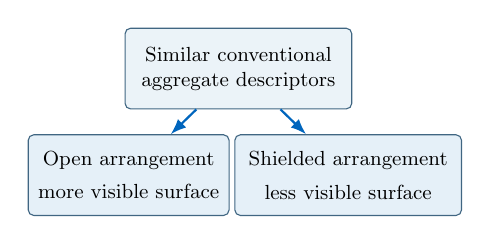
\begin{tikzpicture}[scale=.82,transform shape]
        \node[box,text width=3.3cm,minimum height=1.25cm] (same) at (0,1.65)
          {Similar conventional\\aggregate descriptors};
        \node[physicsbox,text width=2.9cm,minimum height=1.25cm] (a) at (-1.7,0)
          {Open arrangement\\[1ex] more visible surface};
        \node[physicsbox,text width=3.3cm,minimum height=1.25cm] (b) at (1.7,0)
          {Shielded arrangement\\[1ex] less visible surface};
        \draw[arr] (same) -- (a);
        \draw[arr] (same) -- (b);
      \end{tikzpicture}
  \end{columns}
  \vspace{.2cm}
  \takeaway{A useful morphology descriptor must distinguish structures that integral scalars treat as similar.}
\end{frame}

% -----------------------------------------------------------------------------
\begin{frame}{Testing the structural workflow before oxygen simulations}
  \question{Can a particle-contact graph be compressed without losing the information needed to predict geometric exposure?}
  \vspace{.45cm}
  \centering
  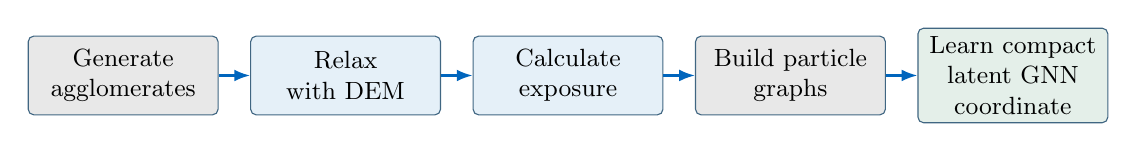
\begin{tikzpicture}[node distance=4mm]
    \node[databox,text width=2.2cm] (gen) {Generate\\agglomerates};
    \node[physicsbox,text width=2.2cm,right=of gen] (dem) {Relax\\with DEM};
    \node[physicsbox,text width=2.2cm,right=of dem] (target) {Calculate\\exposure};
    \node[databox,text width=2.2cm,right=of target] (graph) {Build particle\\graphs};
    \node[outputbox,text width=2.2cm,right=of graph] (gnn) {Learn compact\\ latent GNN \\coordinate};
    \draw[arr] (gen)--(dem);
    \draw[arr] (dem)--(target);
    \draw[arr] (target)--(graph);
    \draw[arr] (graph)--(gnn);
  \end{tikzpicture}
  \vspace{.65cm}
  \begin{columns}[T,onlytextwidth]
    \column{.31\textwidth}\centering
      \hi{Prediction}\\\small How accurately can the graph predict exposure?
    \column{.31\textwidth}\centering
      \hi{Compression}\\\small How many latent variables are needed?
    \column{.31\textwidth}\centering
      \hi{Interpretation}\\\small What structural information is retained?
  \end{columns}
\end{frame}

\section[Exposure target]{Agglomerate generation and exposure target}
\begin{frame}{}
  \vfill
  {\large\color{tumgray}Section 2 of 5}\par\vspace{0.4cm}
  {\LARGE\color{tumblue}\textbf{Agglomerate generation and exposure target}}\par\vspace{0.5cm}
  {\large From synthetic particle structures to a continuous accessibility measure}
  \vfill
\end{frame}

% -----------------------------------------------------------------------------
\begin{frame}{The data set separates size, morphology and random realization}
  \begin{columns}[c,onlytextwidth]
    \column{.48\textwidth}
      \begin{align*}
        N &= k_f\left(\frac{R_g}{r_p}\right)^{D_f},\\[.3em]
        3\ d_p &\times 3\ N \times 3\ \text{morphologies}
        \times 5\ \text{realizations}=135.
      \end{align*}
      \small
      $N$: particle count; $R_g$: radius of gyration;\\ $r_p$: particle radius;\\
      $D_f$: requested fractal dimension;\\ $k_f$: requested fractal prefactor.
    \column{.48\textwidth}
      \begin{table}
        \centering\small
        \begin{tabular}{lcc}
          \toprule
          Morphology & $D_f$ & $k_f$\\
          \midrule
          Open & 1.8 & 1.3\\
          Intermediate & 2.2 & 1.1\\
          Compact & 2.6 & 0.8\\
          \bottomrule
        \end{tabular}
      \end{table}
      \vspace{.2cm}
      \small Each design point contains five \\ independently generated particle arrangements.
  \end{columns}
  \vspace{.3cm}
  \takeaway{The three morphology classes use paired $D_f$ and $k_f$ settings; their individual effects cannot be separated here.}
  \slidesource{Agglomerate generation: Filippov et al. (2000); hierarchical implementation: Skorupski et al. (2014).}
\end{frame}

% -----------------------------------------------------------------------------
\begin{frame}{The ensemble contains visibly different particle arrangements}
  \begin{columns}[T,onlytextwidth]
    \column{.32\textwidth}\centering
      \safeimage{./figures/open.png}{\linewidth}{4.5cm}\\%[-.2em]
      \hi{Open}\\[-.15em]
      \scriptsize $(D_f,k_f)=(1.8,1.3)$
    \column{.32\textwidth}\centering
      \safeimage{./figures/intermediate.png}{\linewidth}{4.5cm}\\%[-.2em]
      \hi{Intermediate}\\[-.15em]
      \scriptsize $(D_f,k_f)=(2.2,1.1)$
    \column{.32\textwidth}\centering
      \safeimage{./figures/compact.png}{\linewidth}{4.5cm}\\%[-.2em]
      \hi{Comparatively compact}\\%[-.15em]
      \scriptsize $(D_f,k_f)=(2.6,0.8)$
  \end{columns}
  \vspace{.15cm}
  \takeaway{All three examples have $N=200$ and $d_p=2\,\mu\mathrm{m}$;\\ colour denotes particle-level exposure from 0.2 to 0.8}
\end{frame}

% -----------------------------------------------------------------------------
\begin{frame}{DEM relaxation turns generated geometry into a physical structure}
  \begin{columns}[c,onlytextwidth]
    \column{.46\textwidth}\centering
      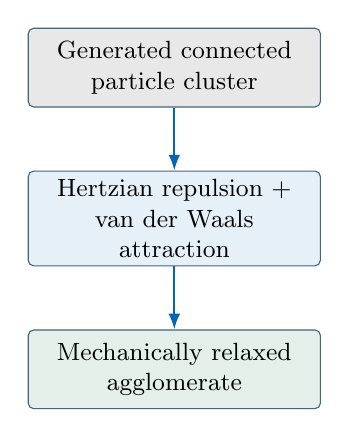
\begin{tikzpicture}[node distance=8mm]
        \node[databox,text width=3.5cm] (initial) {Generated connected\\particle cluster};
        \node[physicsbox,text width=3.5cm,below=of initial] (forces) {Hertzian repulsion +\\van der Waals attraction};
        \node[outputbox,text width=3.5cm,below=of forces] (relaxed) {Mechanically relaxed\\agglomerate};
        \draw[arr] (initial)--(forces);
        \draw[arr] (forces)--(relaxed);
      \end{tikzpicture}
    \column{.50\textwidth}
      \hi{Why relax the structures?}
      \begin{itemize}
        \item Remove small overlaps and force imbalance from generation.
        \item Test whether the cluster remains mechanically connected.
        \item Obtain the final contact geometry used by the graph.
      \end{itemize}
      \vspace{.2cm}
      \hi{Quality checks}
      \begin{itemize}
        \item low residual kinetic energy;
        \item one connected component;
        \item consistent particle and contact output.
      \end{itemize}
  \end{columns}
\end{frame}

% -----------------------------------------------------------------------------
\begin{frame}{Ray tracing measures unobstructed particle directions}
  \centering
  \resizebox{0.60\textwidth}{!}{%
  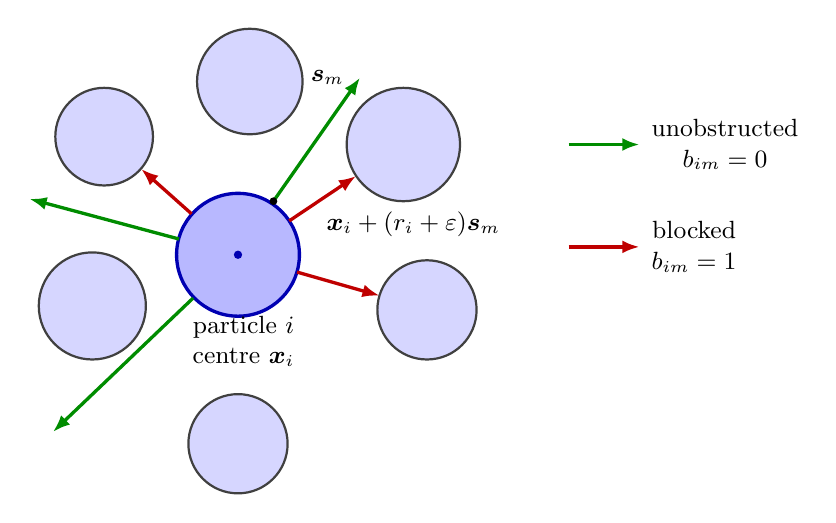
\begin{tikzpicture}[
    x=1cm,y=1cm,
    particle/.style={draw=black!75,thick,fill=blue!16},
    tested/.style={draw=blue!70!black,very thick,fill=blue!28},
    clear ray/.style={-{Latex[length=2.2mm]},very thick,green!55!black},
    blocked ray/.style={-{Latex[length=2.2mm]},very thick,red!75!black},
    label text/.style={font=\small,align=center}
  ]
    \foreach \x/\y/\r in {
      4.55/0.55/0.63,4.25/2.65/0.72,2.30/3.45/0.67,
      0.45/2.75/0.62,0.30/0.60/0.68,2.15/-1.15/0.63}
      \draw[particle] (\x,\y) circle (\r);

    \coordinate (C) at (2.15,1.25);
    \draw[tested] (C) circle (0.78);
    \fill[blue!70!black] (C) circle (1.5pt);
    \node[label text,below right=6.5mm and -7mm of C]
      {particle $i$\\centre $\boldsymbol{x}_i$};

    \draw[clear ray] (2.6,1.93) -- (3.70,3.50);
    \draw[clear ray] (1.40,1.45) -- (-0.50,1.96);
    \draw[clear ray] (1.58,0.70) -- (-0.20,-1.00);

    \draw[blocked ray] (2.90,1.03) -- (3.95,0.73);
    \draw[blocked ray] (2.80,1.68) -- (3.65,2.25);
    \draw[blocked ray] (1.56,1.77) -- (0.92,2.34);

    \fill[black] (2.6,1.93) circle (1.4pt);
    \node[label text,above right=1mm and 10mm of C]
      {$\boldsymbol{x}_i+(r_i+\varepsilon)\boldsymbol{s}_m$};
    \node[label text,right] at (2.95,3.5) {$\boldsymbol{s}_m$};

    \draw[clear ray] (6.35,2.65) -- (7.25,2.65);
    \node[label text,right] at (7.28,2.65)
      {unobstructed\\$b_{im}=0$};
    \draw[blocked ray] (6.35,1.35) -- (7.25,1.35);
    \node[label text,right] at (7.28,1.35)
      {blocked\\$b_{im}=1$};
  \end{tikzpicture}}
  \vspace{-.10cm}
  \takeaway{The calculation uses 512 approximately uniform directions over the full sphere; only a 2D subset is shown.}
\end{frame}

% -----------------------------------------------------------------------------
\begin{frame}{Exposure is a number between zero and one}
  \begin{columns}[c,onlytextwidth]
    \column{.52\textwidth}
      \begin{align*}
        a_i^{\mathrm{geo}}
          &=\frac{1}{M}\sum_{m=1}^{M}(1-b_{im}),\\[.45em]
        \overline a_{\mathrm{geo}}
          &=\frac{1}{N}\sum_{i=1}^{N}a_i^{\mathrm{geo}}.
      \end{align*}
      \small
      $M=512$: sampled ray directions;\\
      $b_{im}$: obstruction indicator for ray $m$ of particle $i$;\\
      $N$: number of particles.
    \column{.44\textwidth}
      \begin{block}{Particle-level meaning}
        $a_i^{\mathrm{geo}}=0$: every sampled direction is blocked.\\[.4em]
        $a_i^{\mathrm{geo}}=1$: every sampled direction is unobstructed.
      \end{block}
      \vspace{.3cm}
      \begin{block}{Aggregate target}
        $\overline a_{\mathrm{geo}}$ is the mean exposure over all particles.
      \end{block}
  \end{columns}
  \vspace{.2cm}
  \takeaway{Exposure is a geometric line-of-sight proxy---not yet oxygen diffusion, uptake or reaction.}
\end{frame}

% -----------------------------------------------------------------------------
% -----------------------------------------------------------------------------
\begin{frame}{Why predict geometric exposure?}
	
	\begin{columns}[T,onlytextwidth]
		\small
		\column{0.48\textwidth}
		\hi{Closer to the uptake mechanism}
		
		\begin{itemize}
			\item Geometric exposure describes the particle surface that is potentially
			accessible from the surroundings.
			
			\item It is therefore directly relevant to possible oxygen uptake.
			
			\item Porosity and fractal dimension describe the overall structure, but
			not the accessible surface directly.
			
			\item An additional  model is needed to connect them
			to oxygen uptake.
		\end{itemize}
		
		\column{0.48\textwidth}
		\hi{Better suited to the present data set}
		
		\begin{itemize}\itemsep0.1ex
			\item The data set contains 135 agglomerates but only three prescribed
			fractal dimension classes ($D_f=1.8, 2.2, 2.6$)
			
			\item This is insufficient for learning a general relationship between
			particle structure and fractal dimension.
			
			\item Geometric exposure varies continuously among the 135 agglomerates.
			
			\item It also distinguishes random realizations belonging to the same
			morphology class.
		\end{itemize}
		
	\end{columns}
	
	\vspace{-0.1cm}
	\takeaway{\small Geometric exposure is a continuous and uptake-relevant target;
		porosity and $D_f$ remain useful structural descriptors.}
	
\end{frame}

\section[Graph method]{Graph model and validation method}
\begin{frame}{}
  \vfill
  {\large\color{tumgray}Section 3 of 5}\par\vspace{0.4cm}
  {\LARGE\color{tumblue}\textbf{Graph model and validation method}}\par\vspace{0.5cm}
  {\large From particle contacts to leakage-free graph learning}
  \vfill
\end{frame}

% -----------------------------------------------------------------------------
\begin{frame}{The relaxed agglomerate becomes a particle-contact graph}
  \begin{columns}[c,onlytextwidth]
    \column{.45\textwidth}\centering
      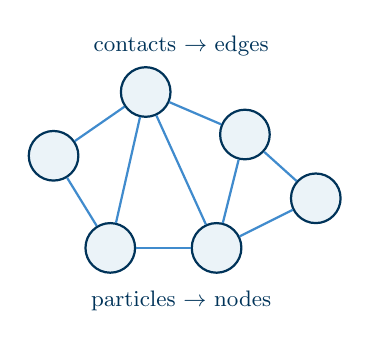
\begin{tikzpicture}[scale=.9,transform shape]
        \foreach \name/\x/\y in {a/0/1.8,b/1.3/2.7,c/2.7/2.1,d/.8/.5,e/2.3/.5,f/3.7/1.2}{
          \node[circle,draw=tumdark,thick,fill=tumlight,minimum size=7mm] (\name) at (\x,\y) {};
        }
        \foreach \u/\v in {a/b,b/c,a/d,b/d,b/e,c/e,c/f,e/f,d/e}
          \draw[thick,tumblue!75] (\u)--(\v);
        \node[font=\small,tumdark] at (1.8,-.25) {particles $\rightarrow$ nodes};
        \node[font=\small,tumdark] at (1.8,3.35) {contacts $\rightarrow$ edges};
      \end{tikzpicture}
    \column{.51\textwidth}
      \hi{Node information}
      \begin{itemize}
        \item radial position: $|\boldsymbol{x}_i-\boldsymbol{x}_c|/R_g$;
        \item coordination number: $z_i$.
      \end{itemize}
      \hi{Edge information}
      \begin{itemize}
        \item normalized centre distance: $d_{ij}/d_{\mathrm{ref}}$;
        \item normalized relative-position vector.
      \end{itemize}
      \small Only geometrically touching or numerically near-touching pairs are retained.
  \end{columns}
  \vspace{.15cm}
  \takeaway{The graph preserves local neighbourhoods and the arrangement of particles across the complete agglomerate.}
\end{frame}

% -----------------------------------------------------------------------------
\begin{frame}{The GNN compresses the whole graph into one learned coordinate}
  \centering
  
  \vspace*{0.5cm}
  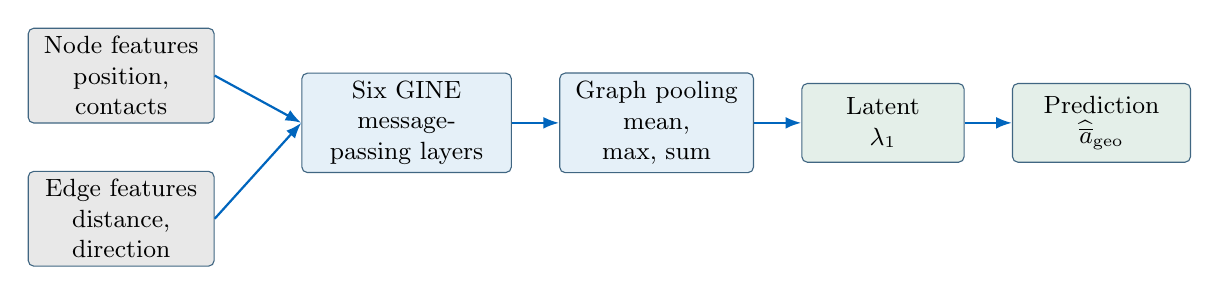
\begin{tikzpicture}[node distance=6mm]
    \node[databox,text width=2.15cm] (node) {Node features\\position, contacts};
    \node[databox,text width=2.15cm,below=6mm of node] (edge) {Edge features\\distance, direction};
    \node[physicsbox,text width=2.45cm,right=11mm of node,yshift=-6mm] (mp) {Six GINE\\message-passing layers};
    \node[physicsbox,text width=2.25cm,right=of mp] (pool) {Graph pooling\\mean, max, sum};
    \node[outputbox,text width=1.85cm,right=of pool] (latent) {Latent\\$\lambda_1$};
    \node[outputbox,text width=2.05cm,right=of latent] (pred) {Prediction\\$\widehat{\overline a}_{\mathrm{geo}}$};
    \draw[arr] (node.east)--(mp.west);
    \draw[arr] (edge.east)--(mp.west);
    \draw[arr] (mp)--(pool);
    \draw[arr] (pool)--(latent);
    \draw[arr] (latent)--(pred);
  \end{tikzpicture}
  \vspace{-.15cm}
  \begin{columns}[T,onlytextwidth]
    \column{.31\textwidth}\centering
      \hi{Messages}\\\small combine each particle with its neighbours.
    \column{.31\textwidth}\centering
      \hi{Pooling}\\\small produces one representation per agglomerate.
    \column{.31\textwidth}\centering
      \hi{Bottleneck}\\\small forces the useful information into $\lambda_1$.
  \end{columns}
  \vspace{.2cm}
  \takeaway{No separately calculated aggregate descriptor is supplied to the latent coordinate or prediction head.}
\end{frame}

% -----------------------------------------------------------------------------
\begin{frame}{Grouped cross-validation tests unseen parameter combinations}
  \begin{columns}[c,onlytextwidth]
    \column{.51\textwidth}
      \hi{Grouping rule}
      \begin{itemize}
        \item The 135 agglomerates form 27 parameter groups; each group contains
          five realizations with the same $(d_p,N,D_f,k_f)$ setting.
        \item The 27 complete groups are distributed among five folds.
        \item In each run, one fold is tested and the other four are used for
          training. A group is never divided between them.
      \end{itemize}
    \column{.45\textwidth}\centering
      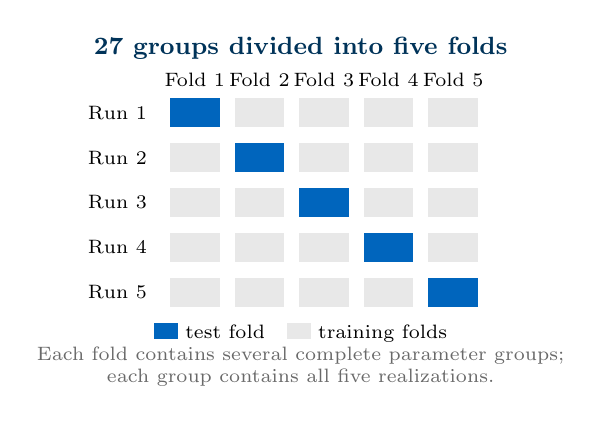
\begin{tikzpicture}[x=.82cm,y=.57cm]
        \node[font=\small\bfseries,tumdark] at (2.05,5.80)
          {27 groups divided into five folds};
        \foreach \f in {1,...,5}{
          \node[font=\scriptsize] at ({\f-0.59},5.10) {Fold \f};
        }
        \foreach \r in {1,...,5}{
          \node[font=\scriptsize,anchor=east] at (-.18,{5-\r+.36}) {Run \r};
          \foreach \f in {1,...,5}{
            \ifnum\r=\f\def\cc{tumblue}\else\def\cc{datagray}\fi
            \fill[\cc] ({\f-1},{5-\r}) rectangle ++(.82,.72);
            \draw[white,line width=1.2pt]
              ({\f-1},{5-\r}) rectangle ++(.82,.72);
          }
        }
        \node[font=\scriptsize] at (2.05,-.55)
          {\textcolor{tumblue}{\rule{3mm}{2mm}} test fold\quad
           \textcolor{datagray}{\rule{3mm}{2mm}} training folds};
        \node[font=\scriptsize,tumgray,align=center] at (2.05,-1.30)
          {Each fold contains several complete parameter groups;\\
           each group contains all five realizations.};
      \end{tikzpicture}
  \end{columns}
  \vspace{.25cm}
  \takeaway{Every reported prediction is out-of-fold: it comes from a model that did not train on that parameter group.}
\end{frame}

\section[Results]{Results and interpretation}
\begin{frame}{}
  \vfill
  {\large\color{tumgray}Section 4 of 5}\par\vspace{0.4cm}
  {\LARGE\color{tumblue}\textbf{Results and interpretation}}\par\vspace{0.5cm}
  {\large Predictive accuracy and what the latent coordinate retains}
  \vfill
\end{frame}

% -----------------------------------------------------------------------------
\begin{frame}{One graph coordinate predicts exposure with $R^2=0.954$}
  \begin{columns}[T,onlytextwidth]
    \column{.56\textwidth}\centering
      \safeimage{./figures/mean_geometric_exposure_oof_performance.png}{\linewidth}{6.25cm}
    \column{.45\textwidth}
      \vspace{.35cm}
      \begin{block}{Grouped out-of-fold performance}
        \centering
        \large
        RMSE $=0.0160$\\[.35em]
        MAE $=0.0128$\\[.35em]
        $R^2=0.954$
      \end{block}
      \vspace{.3cm}
      \small Points close to the diagonal indicate agreement between calculated and GNN-predicted mean exposure.
  \end{columns}
  
  \vspace*{-0.8cm}
  \takeaway{A one-dimensional bottleneck retains nearly all information needed for this specific prediction task.}
\end{frame}

% -----------------------------------------------------------------------------
\begin{frame}{Prediction accuracy remains consistent across the five test folds}
  \begin{columns}[c,onlytextwidth]
    \column{.58\textwidth}\centering
      \safeimage{./figures/mean_geometric_exposure_fold_rmse.png}{\linewidth}{5.15cm}
    \column{.38\textwidth}
      \hi{Fold-specific RMSE}
      \begin{itemize}
        \item Fold 1: 0.0194
        \item Fold 2: 0.0128
        \item Fold 3: 0.0133
        \item Fold 4: 0.0162
        \item Fold 5: 0.0172
      \end{itemize}
      \small The dashed line in the figure denotes the mean fold RMSE.
  \end{columns}
  \vspace{.15cm}
  \takeaway{The performance is not produced by one unusually easy split.}
\end{frame}

% -----------------------------------------------------------------------------
\begin{frame}{The particle graph adds information beyond conventional scalars}
  \small
  \begin{table}
    \centering
    \begin{tabular}{lrrr}
      \toprule
      Model or input & RMSE & MAE & $R^2$\\
      \midrule
      \textbf{Pure-graph GNN} & \textbf{0.0160} & \textbf{0.0128} & \textbf{0.954}\\
      Six calculated descriptors, linear & 0.0209 & 0.0183 & 0.922\\
      Six calculated descriptors, random forest & 0.0235 & 0.0168 & 0.902\\
      Requested $D_f$ and $k_f$, linear & 0.0472 & 0.0399 & 0.604\\
      Best individual descriptor & 0.0524 & 0.0383 & 0.511\\
      Particle count, linear & 0.0687 & 0.0582 & 0.160\\
      \bottomrule
    \end{tabular}
  \end{table}
  \vspace{.55cm}
  \begin{columns}[T,onlytextwidth]
    \column{.48\textwidth}\centering
      \hi{$D_f+k_f$ are informative}\\[-.1em]
      \small but they describe only the prescribed morphology class.
    \column{.48\textwidth}\centering
      \hi{The graph is more precise}\\[-.1em]
      \small because it sees realization-, size- and relaxation-dependent structure.
  \end{columns}
\end{frame}

% -----------------------------------------------------------------------------
\begin{frame}{The learned coordinate is task-specific, not a renamed scalar}
  \begin{columns}[c,onlytextwidth]
    \column{.50\textwidth}
      \hi{Strongest monotonic associations}
      \begin{table}
        \centering\small
        \begin{tabular}{lr}
          \toprule
          Descriptor & Spearman $\rho$\\
          \midrule
          Requested $D_f$ & $-0.800$\\
          Requested $k_f$ & $+0.800$\\
          Number of contacts & $-0.596$\\
          Particle count & $-0.544$\\
          Maximum coordination & $-0.541$\\
          \bottomrule
        \end{tabular}
      \end{table}
    \column{.46\textwidth}
      \begin{itemize}
        \item One scalar alone does not reconstruct the learned coordinate well.
        \item Several morphology measures together reconstruct it accurately.
        \item Its sign is arbitrary; its encoded ordering and predictive content matter.
      \end{itemize}
  \end{columns}
  \vspace{.2cm}
  \takeaway{$\lambda_1$ combines several structural attributes in the direction most useful for predicting exposure.}
\end{frame}

\section[Conclusions]{Conclusions and next steps}
\begin{frame}{}
  \vfill
  {\large\color{tumgray}Section 5 of 5}\par\vspace{0.4cm}
  {\LARGE\color{tumblue}\textbf{Conclusions and next steps}}\par\vspace{0.5cm}
  {\large What the evidence supports and what remains to validate}
  \vfill
\end{frame}

% -----------------------------------------------------------------------------
\begin{frame}{The present result is a structural proof of concept}
  \begin{columns}[T,onlytextwidth]
    \column{.47\textwidth}
      \hi{What has been demonstrated}
      \begin{itemize}
        \item stable DEM-to-graph workflow for 135 agglomerates;
        \item physically interpretable ray-based exposure target;
        \item accurate exposure prediction with one latent coordinate;
        \item improvement over prescribed and calculated scalar descriptors.
      \end{itemize}
    \column{.49\textwidth}
      \hi{What has not yet been demonstrated}
      \begin{itemize}
        \item oxygen diffusion through tortuous pores;
        \item flow-induced transport around or within an agglomerate;
        \item oxygen consumption and reaction--transport coupling;
        \item direct prediction of biological activity.
      \end{itemize}
  \end{columns}
  \vspace{.3cm}
  \takeaway{Geometric exposure is a useful screening target, but its relationship to oxygen uptake must be validated.}
\end{frame}

% -----------------------------------------------------------------------------
\begin{frame}{Resolved oxygen transport is the decisive next test}
  \centering
  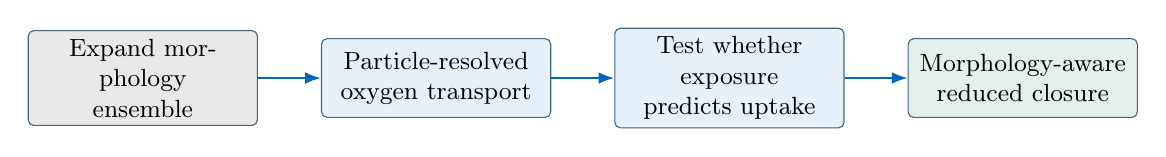
\begin{tikzpicture}[node distance=8mm]
    \node[databox,text width=2.7cm] (expand) {Expand morphology\\ensemble};
    \node[physicsbox,text width=2.7cm,right=of expand] (transport) {Particle-resolved\\oxygen transport};
    \node[physicsbox,text width=2.7cm,right=of transport] (validate) {Test whether exposure\\predicts uptake};
    \node[outputbox,text width=2.7cm,right=of validate] (closure) {Morphology-aware\\reduced closure};
    \draw[arr] (expand)--(transport);
    \draw[arr] (transport)--(validate);
    \draw[arr] (validate)--(closure);
  \end{tikzpicture}
  \vspace{.65cm}
  \begin{columns}[T,onlytextwidth]
    \column{.31\textwidth}\centering
      \hi{Geometry checks}\\\small ray-number convergence and finite probe radius
    \column{.31\textwidth}\centering
      \hi{Transport targets}\\\small uptake, response time and oxygen-limited fraction
    \column{.31\textwidth}\centering
      \hi{Model decision}\\\small retain exposure or enrich the graph with transport information
  \end{columns}
\end{frame}

% -----------------------------------------------------------------------------
\begin{frame}{The detailed graph provides a compact bridge to transport models}
  \vspace{.3cm}
  \question{A single learned graph coordinate predicts ray-based geometric exposure with grouped out-of-fold $R^2=0.954$.}
  \vspace{.55cm}
  \begin{columns}[T,onlytextwidth]
    \column{.31\textwidth}\centering
      \hi{Meaningful target}\\[.25em]
      \small Exposure quantifies directional surface obstruction from 0 to 1.
    \column{.31\textwidth}\centering
      \hi{Useful compression}\\[.25em]
      \small One latent coordinate retains task-relevant graph information.
    \column{.31\textwidth}\centering
      \hi{Clear next step}\\[.25em]
      \small Validate the structural proxy against resolved oxygen transport.
  \end{columns}
  \vspace{.65cm}
  \takeaway{The proof of concept supports using graph-based morphology descriptors in the planned oxygen-transport study.}
\end{frame}

\end{document}
